\documentclass{beamer}

\usepackage{xcolor}
\usepackage{graphicx}
\usepackage{varwidth}
% \usepackage{caption}

\usepackage{subcaption}
\usepackage{media9}
\usepackage{multimedia}

\usepackage{amsfonts,amsmath,amssymb}
\usepackage{blkarray,booktabs,bigstrut}

\usepackage{pgfplots}
\usepackage{tikz}
\usepackage{filecontents}
\usepackage{lmodern}

\usetikzlibrary{hobby}
\usetikzlibrary{decorations.shapes}
\usetikzlibrary{shadows.blur}

\definecolor{NvidiaGreen}{RGB}{118, 185, 0}

\usetheme{Madrid}
\setbeamertemplate{navigation symbols}{}

% Set the colors for various Beamer elements
\setbeamercolor{title}{fg=black, bg=NvidiaGreen} 
\setbeamercolor{frametitle}{fg=black, bg=NvidiaGreen} 
\setbeamercolor{item}{fg=black, bg=NvidiaGreen} 
\setbeamercolor{section in toc}{fg=black, bg=NvidiaGreen}
\setbeamercolor{author}{fg=white, 
        % bg=NvidiaGreen
    }
\setbeamercolor{date}{fg=white, 
        % bg=NvidiaGreen
    }

% Set the background to white for a clean presentation
\setbeamercolor{background canvas}{bg=white}

% #########################################################################################
% #########################################################################################
% Title
% #########################################################################################
% #########################################################################################

\begin{document}
{
\setbeamertemplate{background} 
{
    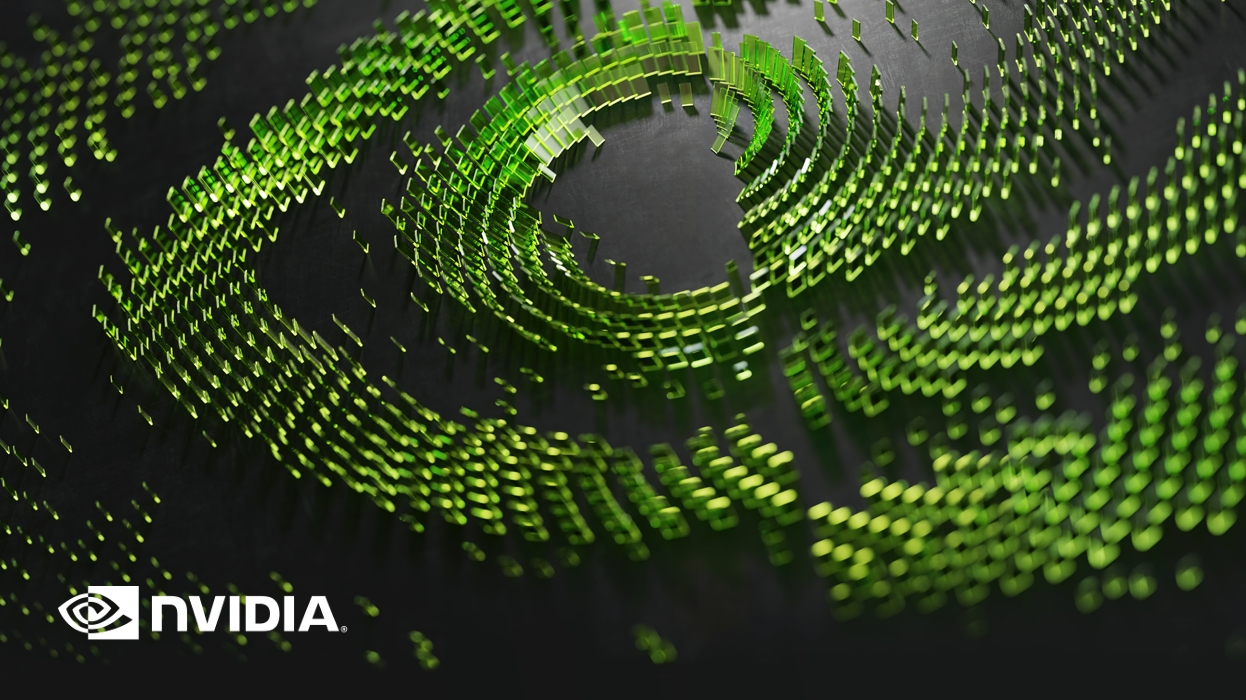
\includegraphics[width=\paperwidth,height=\paperheight]{images/Screenshot_9-12-2024_212019_.jpeg}
}
\title{\textbf{Computation and Neural Manifolds}}
\author[]{\textbf{Renan Monteiro Barbosa}}
% \date{\today}
\date[]{\textbf{2025}}
\maketitle
}

% #########################################################################################
% #########################################################################################
% Slide 1 - Intro
% #########################################################################################
% #########################################################################################

\section{Neural Manifolds}
\begin{frame}
\frametitle{\textbf{Neural Manifolds}}

Neural manifolds are being uncovered in many tasks aacrros the brain that help explain cognition

\begin{itemize}
    \item What are neural manifolds?
    \begin{enumerate}
        \item Neural manifolds are abstractions of neural trajectories, neurodynamical structure, often low-dimensional, in high-dimensional neural activity.
    \end{enumerate}
    \item What do neural manifolds do ?
    \begin{enumerate}
        \item Neural manifolds provide evidence for what is being computed by the brain.
        \item Neural manifolds provide evidence for how the brain computes.
    \end{enumerate}
\end{itemize}


\end{frame}

% #########################################################################################
% #########################################################################################
% Slide 2 - Neural Activity
% #########################################################################################
% #########################################################################################

\section{Neural Activity}
\begin{frame}
\frametitle{\textbf{Neural Activity} }

Neural activity can be described as a high-dimensional neural spcace.

%  TODO - draw the Neural N-Space and the Manifold 3-Space

We start at some prat of the brain, the dimensionality is the number of neurons on that part, and each dimension is the firing rate of those neurons. The trajectory is the evolution of time 

Manifolds are the abstraction fo the Neural N-Space to represent the activity over time

% In neural N-space, the activity of a neural network is described by a vector where each dimension represents the activity of a single neuron. This vector, or neural state, can be visualized as a point in an N-dimensional space, where N is the number of neurons. This framework allows for a more comprehensive understanding of network activity, including how it evolves and how different neurons interact. 

% N-Dimensional State Space:
% Each neuron's activity (e.g., firing rate) contributes to a coordinate in this N-dimensional space. The instantaneous activity of all neurons collectively forms a point within this space, representing the current state of the network. 

% Neural States and Manifolds:
% Neural activity is often not random; it tends to cluster around specific points or regions within the state space. These clusters or regions are known as intrinsic manifolds, representing the typical or relevant activity patterns of the network. 

% Predicting and Interpreting Activity:
% By understanding the dynamics within this N-space, it becomes possible to predict future activity patterns or interpret the computational role of specific neural regions. 


\end{frame}

% #########################################################################################
% #########################################################################################
% Slide 3 - Intro
% #########################################################################################
% #########################################################################################

\section{Manifolds}
\begin{frame}
\frametitle{\textbf{Manifolds} }

Manifolds can be described as subspaces of vector spaces.

each vector is called the Basis vector

Basis Vectors: every point on manifold is a linear combination of these vectors.

%  TODO need work on this slide

\centering
\begin{minipage}{1\textwidth}
    \centering
    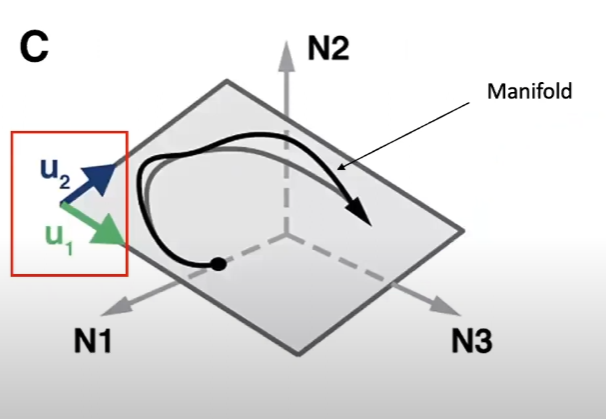
\includegraphics[width=0.4\textwidth]{images/gallego_et_al-2017_01.PNG} % Replace with your image file
    \captionof{figure}{manifold}
\end{minipage}

Trajectory of time-varying population activity in the neural space of the three recorded neurons (black). The trajectory is mostly confined to the neural manifold, a plane shown in gray and spanned by the neural modes $u_1$ and $u_2$.

\end{frame}

% #########################################################################################
% #########################################################################################
% Slide 4 - Neural Manifolds
% #########################################################################################
% #########################################################################################

\section{Neural Manifolds}
\begin{frame}
\frametitle{\textbf{Neural Manifolds} }
% repeat the intro slide
Neural manifolds are being uncovered in many tasks across the brain that help explain cognition.

\begin{itemize}
    \item What are neural manifolds?
    \begin{enumerate}
        \item Neural manifolds are abstractions of neural trajectories, neurodynamical structure, often low-dimensional, in high-dimensional neural activity.
    \end{enumerate}
    \item What do neural manifolds do ?
    \begin{enumerate}
        \item Neural manifolds provide evidence for what is being computed by the brain.
        \item Neural manifolds provide evidence for how the brain computes.
    \end{enumerate}
\end{itemize}


\end{frame}

% #########################################################################################
% #########################################################################################
% Slide 5 - Temporal interval estimation
% #########################################################################################
% #########################################################################################

\section{Temporal interval estimation}
\begin{frame}
\frametitle{\textbf{Temporal interval estimation} }

In the temporal interval estimation task, monkeys estiamte the duration of a temporal interval.

% TODO - add picture form Sohn et al. 2019

\centering
\begin{minipage}{1\textwidth}
    \centering
    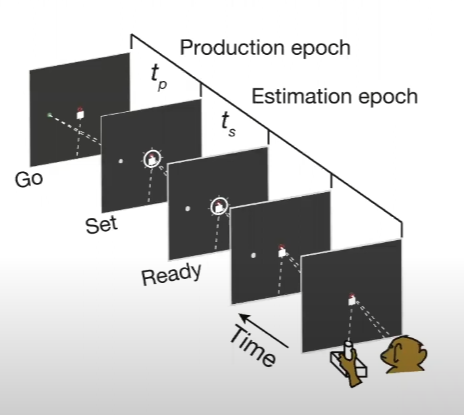
\includegraphics[width=0.4\textwidth]{images/Sohn_et_al-2019_01.PNG} % Replace with your image file
    \captionof{figure}{temporal interval estimation}
\end{minipage}

Schematic of a single trial of the ReadySet-Go task. The animal has to estimate a sample interval, ts, between Ready and Set (estimation epoch), and produce a matching interval, tp, after Set with a delayed response (Go) via a saccade or a movement of the joystick (production epoch).

\end{frame}

% #########################################################################################
% #########################################################################################
% Slide 6 - What counts as evidence for what is computed
% #########################################################################################
% #########################################################################################

\section{what is being computed?}
\begin{frame}
\frametitle{\textbf{what is being computed?} }
What counts as evidence for what is being computed ?

Generally, physical systems provide evidence for what is computed if:

\begin{enumerate}
    \item the proposed computation maps on to the behavior
    \item the behavior maps on to the properties of the part
    \item the part maps on to the proposed computation
\end{enumerate}

But first, what was the computation ?

% TODO - maybe here is a good point to reflect on Shagrir and theory of computation
% Can talk about mechanical computers

\end{frame}

% #########################################################################################
% #########################################################################################
% Slide 7 - Bayesian Computation
% #########################################################################################
% #########################################################################################

\section{Bayesian Computation}
\begin{frame}
\frametitle{\textbf{Bayesian Computation} }
A Bayesian computation was hypothesized for estimating intervals.

%  TODO add picture form Sohn et al. 2019

The temporal interval estimation task is being analyzed to discover how the brain is computing.

\centering
\begin{minipage}{1\textwidth}
    \centering
    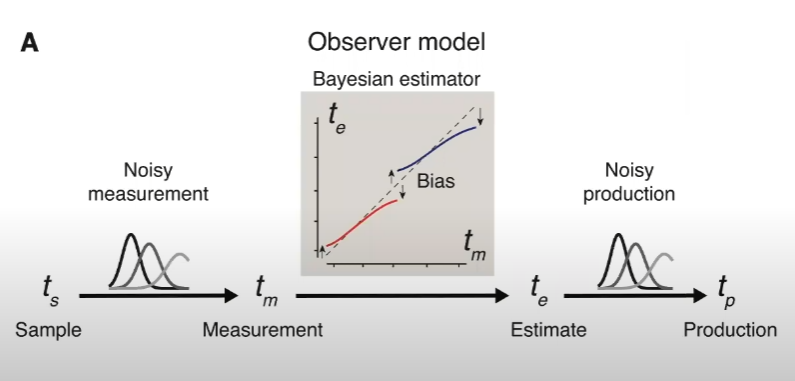
\includegraphics[width=0.4\textwidth]{images/Sohn_et_al-2019_02.PNG} % Replace with your image file
    \captionof{figure}{temporal interval estimation}
\end{minipage}

\end{frame}

% #########################################################################################
% #########################################################################################
% Slide 8 - Behavior on Temporal Estimation Task
% #########################################################################################
% #########################################################################################

\section{Behavior on Temporal Estimation Task}
\begin{frame}
\frametitle{\textbf{Behavior on Temporal Estimation Task} }

Cool graphs go here
% TODO - Add the image from Sohn et al. 2019

\centering
\begin{minipage}{1\textwidth}
    \centering
    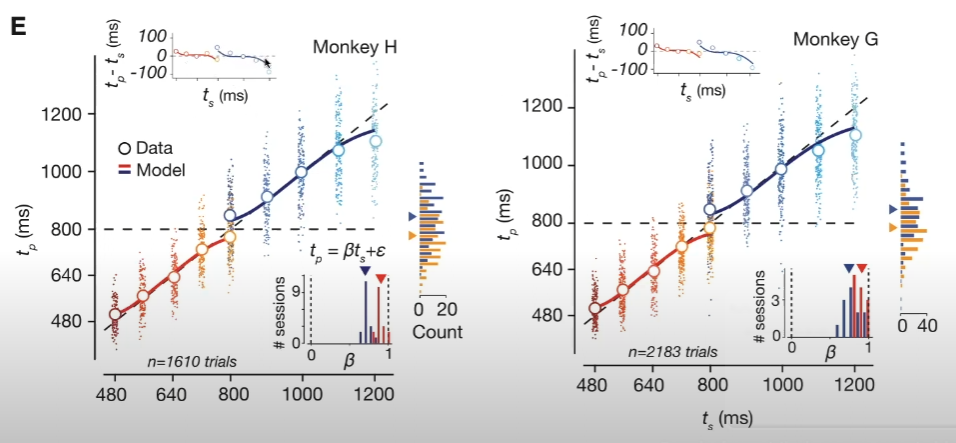
\includegraphics[width=0.4\textwidth]{images/Sohn_et_al-2019_03.PNG} % Replace with your image file
    \captionof{figure}{temporal interval estimation}
\end{minipage}

% Behavior. Top: a representative session for monkey H showing tp pooled across effectors and target directions (small dots, individual trials; large open circles, average tp per ts; solid lines, Bayesian model; diagonal, unity line). The horizontal location of dots was jittered to facilitate visualization. Right: histograms of tp for the overlapping ts (horizontal dashed line) for the two prior conditions (orange, Short; blue, Long; triangles, averages). Top-left inset: average error (i.e., bias) for each ts (circles, data; solid lines, Bayesian model). Bottom-right inset: histogram of regression slopes relating tp to ts across sessions (red, Short; blue, Long; triangles, averages). Bottom: the same as top for monkey G.

\end{frame}

% #########################################################################################
% #########################################################################################
% Slide 9 - what is being computed?
% #########################################################################################
% #########################################################################################

\section{what is being computed?}
\begin{frame}
\frametitle{\textbf{what is being computed?} }
What counts as evidence for what is being computed ?

Generally, physical systems provide evidence for what is computed if:

\begin{enumerate}
    \item the proposed computation maps on to the behavior
    
    The Bayesian computation maps the bias in estimates of the interval

    \item the behavior maps on to the properties of the part
    
    How about the behaviour part mapping ?

    \item the part maps on to the proposed computation
\end{enumerate}

But first, what was the computation ?

% TODO - maybe here is a good point to reflect on Shagrir and theory of computation
% Can talk about mechanical computers

\end{frame}

% #########################################################################################
% #########################################################################################
% Slide 10 - Neural Manifolds on Temporal Estimation Task
% #########################################################################################
% #########################################################################################

\section{Neural Manifolds on Temporal Estimation Task}
\begin{frame}
\frametitle{\textbf{Neural Manifolds on Temporal Estimation Task} }

%  TODO - Add image from Sohn et al. 2019

Using Principal component Analysis, we can reduce and project this neural activity in a 3D space formed from the 3 principal components.

So know we can see the behavior maps on the properties of the part, for longer intervals there is a longer manifolds for shorter intervals there is shorter manifolds.

\centering
\begin{minipage}{1\textwidth}
    \centering
    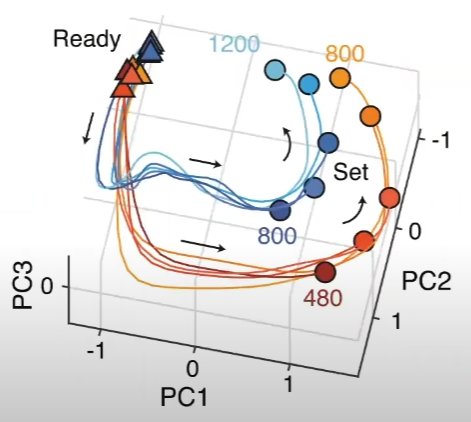
\includegraphics[width=0.4\textwidth]{images/Sohn_et_al-2019_04.PNG} % Replace with your image file
    \captionof{figure}{temporal interval estimation}
\end{minipage}

\end{frame}

% #########################################################################################
% #########################################################################################
% Slide 11 - what is being computed?
% #########################################################################################
% #########################################################################################

\section{what is being computed?}
\begin{frame}
\frametitle{\textbf{what is being computed?} }
What counts as evidence for what is being computed ?

Generally, physical systems provide evidence for what is computed if:

\begin{enumerate}
    \item the proposed computation maps on to the behavior
    
    The Bayesian computation maps the bias in estimates of the interval

    \item the behavior maps on to the properties of the part
    
    the position along the curved manigolds maps the estimate of the interval

    \item the part maps on to the proposed computation
    
    Does the manifolds maps on to the computation?
\end{enumerate}

\end{frame}

% #########################################################################################
% #########################################################################################
% Slide 12 - manifolds maps on to the computation?
% #########################################################################################
% #########################################################################################

\section{manifolds maps on to the computation?}
\begin{frame}
\frametitle{\textbf{manifolds maps on to the computation?} }
Different inputs determine the identity of the manifolds and the position in manifold space.

% TODO - add graph from the Sohn et al 2019
% Need to add the arrows to the Graph 

Different manifolds for different priors

Different states for different intervals within a distribution provide the input to the projection.

\centering
\begin{minipage}{1\textwidth}
    \centering
    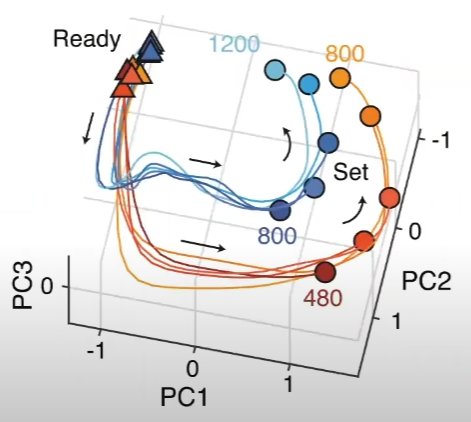
\includegraphics[width=0.4\textwidth]{images/Sohn_et_al-2019_04.PNG} % Replace with your image file
    \captionof{figure}{temporal interval estimation}
\end{minipage}

\end{frame}

% #########################################################################################
% #########################################################################################
% Slide 13 - what is being computed?
% #########################################################################################
% #########################################################################################

\section{what is being computed?}
\begin{frame}
\frametitle{\textbf{what is being computed?} }
What counts as evidence for what is being computed ?

Generally, physical systems provide evidence for what is computed if:

\begin{enumerate}
    \item the proposed computation maps on to the behavior
    
    The Bayesian computation maps the bias in estimates of the interval

    \item the behavior maps on to the properties of the part
    
    the position along the curved manigolds maps the estimate of the interval

    \item the part maps on to the proposed computation
    
    the position along the curved manifold maps the Bayesian computation
\end{enumerate}

\end{frame}

% #########################################################################################
% #########################################################################################
% Slide 14 - Evidence for what is being computed
% #########################################################################################
% #########################################################################################

\section{Evidence for what is being computed}
\begin{frame}
\frametitle{\textbf{Evidence for what is being computed} }
A three-way mapping between computation, part, and behavior is evidence for what is being computed.

The Bayesian computation maps the bias in estimates of the interval, the position along the curved manifolds maps the estimate of the interval, and the position along the curved manigolds maps the Bayesian computation.

Now we know how the Brain computes, can we use the Manifolds as evidence for What the Brain Computes ?

% What is Bayesian Computation
% Approximate Bayesian Computation: Introduction & Insurance Examples
% https://www.youtube.com/watch?v=pwVgIh1495A

\end{frame}

% #########################################################################################
% #########################################################################################
% Slide 15 - How it is being computed?
% #########################################################################################
% #########################################################################################

\section{How it is being computed?}
\begin{frame}
\frametitle{\textbf{How it is being computed?} }

% Might need to break the information on more slides

Manifolds are also evidence for how something is being computed.

How the Bayesian estimates are being computed by neural activity.

The hypothesized computation was a projection from the manifold on to an encoding dimension.

% TODO add iamges from Sohn et al. 2019

\centering
\begin{minipage}{1\textwidth}
    \centering
    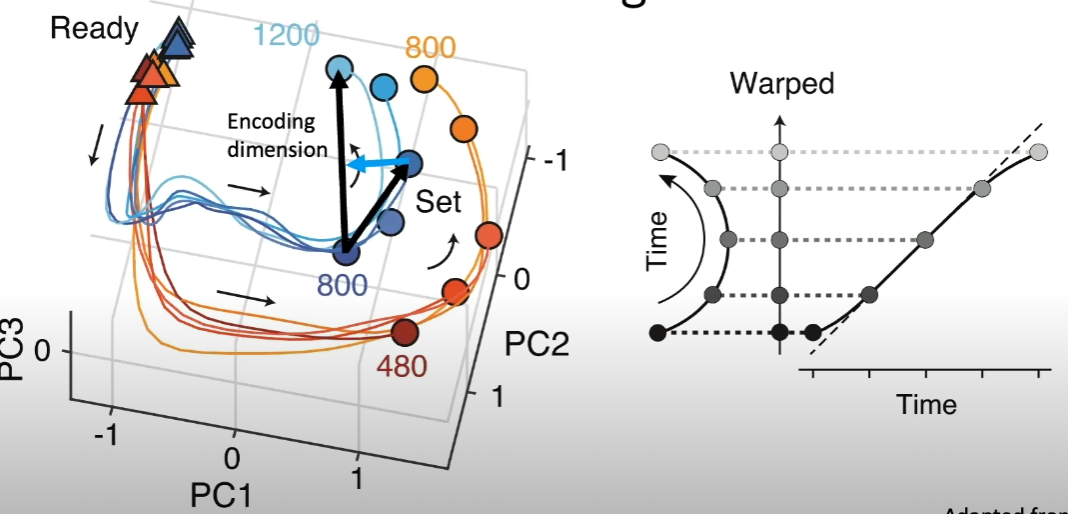
\includegraphics[width=0.2\textwidth]{images/Sohn_et_al-2019_05.PNG} % Replace with your image file
    \captionof{figure}{temporal interval estimation}
\end{minipage}

the second computation was a projection from the manifold onto what they called an encoding dimension.

This encoding Dimension was simply the vector described by the line that connected two points onto the manifold:

\begin{itemize}
    \item The point corresponding to the shortest interval to be estimated in a distribution
    \item The point corresponding to the longest interval in the distribution to be estimated
\end{itemize}

The geometry of projecting a curve onto a line is the compression of the lengths of the arcs along the curve that corresponds to segments of the line. This gives rise to the BIAS

Shorter interval corresponds to shorter length, Longer interval corresponds to longer length.

% TODO - describe a little about Discrete Differential Geometry and build it towrds the Information Geometry.

\end{frame}

% #########################################################################################
% #########################################################################################
% Slide 16 - How it is being computed?
% #########################################################################################
% #########################################################################################

\section{How it is being computed?}
\begin{frame}
\frametitle{\textbf{How it is being computed?} }
Intermediate intervals are mapped onto intermediate points on the manifold.

% TODO add images from Sohn et al 2019

So the differences in the input to the vector projection give rise to differences in speed.

% This is depicted on the Projection onto u graph

x-axis is the projection onto the encoding dimension u and the y-axis is the speed through that manifold space along the curved 2D manifold and there is a law like correlation where the greate the projection onto U slower the speed .

We can observe a preservation in the projections of the relations between the speeds between the output of the computations and the properties of the manifolds and the proposed computation of vector projection

\end{frame}

% #########################################################################################
% #########################################################################################
% Slide 17 - How it is being computed?
% #########################################################################################
% #########################################################################################

\section{How it is being computed?}
\begin{frame}
\frametitle{\textbf{How it is being computed?} }
Manifolds provide evidence for how somehting is being computed.

Points on manifold map onto inputs and points on manifold or in manifold space map onto outputs of computation, and the relations between inputs and outputs of the computation have corresponding relations between points on manifold or in manifold space.

There is a Homomorphism, which is the preservation of relations between the outputs of the proposed computation and there is a corresponding relation in manifold space that preserves those relations.

\end{frame}

% #########################################################################################
% #########################################################################################
% Slide 18 - Objections
% #########################################################################################
% #########################################################################################

\section{Objections}
\begin{frame}
\frametitle{\textbf{Objections} }
Arent all these computations the result of a single neuron activity ?

\end{frame}

% #########################################################################################
% #########################################################################################
% Slide 19 - Example of computation by neurons: perceptual decision making
% #########################################################################################
% #########################################################################################

\section{Example of computation by neurons: perceptual decision making}
\begin{frame}
\frametitle{\textbf{Example of computation by neurons: perceptual decision making} }
Example of computation by neurons: perceptual decision making

% TODO - add images on perceptual decision making

Stage 1: MT - Sensory Evidence

Stage 2: LIP - Accumulated Sensory Evidence

Stage 3: Choice - Categorization of evidence

\end{frame}

% #########################################################################################
% #########################################################################################
% Slide 20 - Objections Reply
% #########################################################################################
% #########################################################################################

\section{Objections Reply}
\begin{frame}
\frametitle{\textbf{Objections Reply} }
Arent all these computations the result of a single neuron activity ?

Reply:

Single Neurons cannot span a >1D space

But manifolds are often 1D

But often they are >1D

\end{frame}

% #########################################################################################
% #########################################################################################
% Slide 21 - Objections
% #########################################################################################
% #########################################################################################

\section{Objections}
\begin{frame}
\frametitle{\textbf{Objections} }

\begin{enumerate}
    \item Arent all these computations the result of a single neuron activity ?
    \item Arent all these computations the result of population activity ?
\end{enumerate}



\end{frame}

% #########################################################################################
% #########################################################################################
% Slide 22 - Objections Reply
% #########################################################################################
% #########################################################################################

\section{Objections Reply}
\begin{frame}
\frametitle{\textbf{Objections Reply} }

\begin{enumerate}
    \item Arent all these computations the result of a single neuron activity ?
    \item Arent all these computations the result of population activity ?
\end{enumerate}

Reply

\begin{itemize}
    \item Different population patterns can result in the same manifold.
    \item Population equivalence classes are not the right type of thing to transform inputs into outputs or to structure dynamics.
    \item What all the elements of the population equivalence class have in common are the dynamics -> collapses into manifold view
\end{itemize}


In other words, different patterns of spiking activity across the population results in the same low dimensional dynamical structure.


In other works, the neural trajectories whose abstractions are the neural manifolds.

This implies that there are not dedicated neurons that encode the manifold dimensions because there is a variety of diversity of population activity patterns that can give rise to it.

\end{frame}

% #########################################################################################
% #########################################################################################
% Slide 23 - Objections
% #########################################################################################
% #########################################################################################

\section{Objections}
\begin{frame}
\frametitle{\textbf{Objections} }

\begin{enumerate}
    \item Arent all these computations the result of a single neuron activity ?
    \item Arent all these computations the result of population activity ?
    \item Arent all these computations the result of other features of the population ?
\end{enumerate}


\end{frame}

% #########################################################################################
% #########################################################################################
% Slide 24 - Objections Reply
% #########################################################################################
% #########################################################################################

\section{Objections Reply}
\begin{frame}
\frametitle{\textbf{Objections Reply} }

\begin{enumerate}
    \item Arent all these computations the result of a single neuron activity ?
    \item Arent all these computations the result of population activity ?
    \item Arent all these computations the result of other features of the population ?
\end{enumerate}

Reply

\begin{itemize}
    \item The weight matrix is not sufficient: difference numbers of neurons and different sets of weights are sufficient for the same manifold.
    \item What difference weight matrices have in common are just those dynamics -> collapses into manifold view.
    \item Similar point applies for other features of population (e.g., noise correlations)
\end{itemize}


\end{frame}

% #########################################################################################
% #########################################################################################
% Slide 25 - Neurocomputational Manifold Hypothesis
% #########################################################################################
% #########################################################################################

\section{Neuraocomputational Manifold Hypothesis}
\begin{frame}
\frametitle{\textbf{Neuraocomputational Manifold Hypothesis} }

NCM - Neural Trajectory n on a manifold m in manifold space S is a computation of a function f over inputs i and outputs o only if there is:

\begin{itemize}
    \item input mapping: neural trajectory n starts on m that maps onto i;
    \item output mapping: neural trajectory n ends at a point in S that maps onto o; and
    \item relation mapping: for every relation R between pairs of i and o of f, there is a relation R' between pairs of points from n on m and in S.
\end{itemize}


\end{frame}

% #########################################################################################
% #########################################################################################
% Slide 26 - Objections
% #########################################################################################
% #########################################################################################

\section{Objections}
\begin{frame}
\frametitle{\textbf{Objections} }

\begin{enumerate}
    \item Arent all these computations the result of a single neuron activity ?
    \item Arent all these computations the result of population activity ?
    \item Arent all these computations the result of other features of the population ?
    \item Manifolds arent real.
\end{enumerate}


\end{frame}

% #########################################################################################
% #########################################################################################
% Slide 27 - Inpute-State-Output Analysis of Computation
% #########################################################################################
% #########################################################################################

\section{Inpute-State-Output Analysis of Computation}
\begin{frame}
\frametitle{\textbf{Inpute-State-Output Analysis of Computation} }

A physical system P implements a CSA M if there is a vectorization of internal states of P into components $\left[s^1, s^2, \cdots\right]$, and a mapping f from the substates $s^j$ into corresponding substates $S^j$ of M, along with similar vectorizations and mapping for inputs and outputs, such that for every state-transition rule $\left(\left[I^1, \cdots, I^k\right],\left[S^1, S^2, \cdots\right]\right) -> \left(\left[S^{\prime 1}, S^{\prime 2}, \cdots\right],\left[O^1, \cdots, O^i\right]\right)$ of M: if P is in internal state $\left[s^1, s^2, \cdots\right]$ and receiving input $\left[i^i, \cdots, i^n\right]$ which map to formal state and input $\left[S^1, S^2, \cdots\right]$ and $\left[I^1, \cdots, I^k\right]$ respectively, this reliably causes it to enter an internal state and produce an output that map to $\left[S^{\prime 1}, S^{\prime 2}, \cdots\right]$ and $\left[O^1, \cdots, O^i\right]$ respectively. 

Chalmers 2011, p.329


\end{frame}

% #########################################################################################
% #########################################################################################
% Slide 28 - Inpute-State-Output Analysis of Computation Reply
% #########################################################################################
% #########################################################################################

\section{Inpute-State-Output Analysis of Computation Reply}
\begin{frame}
\frametitle{\textbf{Inpute-State-Output Analysis of Computation Reply} }

This is different than the computations outlined in the temporal interval estimation that rely on manifolds.

The computation or those trajectories does not rely on these sort of state to state transformations.

Because across different manifolds such as the transformation from the estimation epic one-dimensional manifolds to the production epic two-dimensional may involve state-to-state changes, but it also may involve changes in manifold space altogether.

Also part of the Manifold hypothesis is the preservation of the relations, the homomorphism and that requirement is absent from the Inpute-State-Output Analysis of Computation. Thus this analysis is insufficient.

\end{frame}

% #########################################################################################
% #########################################################################################
% Slide 29 - Input-Output Analysis of Computation
% #########################################################################################
% #########################################################################################

\section{Input-Output Analysis of Computation}
\begin{frame}
\frametitle{\textbf{Input-Output Analysis of Computation} }

Cummins says that "to compute a function g is to execute a program that gives o as its output on input i just in case $g(i) = o$. Computing reduces to program execution, so our problem reduces to explaining what it is to execute a program ... program exectuion involves steps, and to treat each elementary step as a function that the executing system simply satisfies. To execute a program is to satisfy steps" - Cummins 1989, p. 91-92


Temporal Interval estimation cannot be described as program execution 

\end{frame}

% #########################################################################################
% #########################################################################################
% Slide 30 - Modeling Analysis of Computation
% #########################################################################################
% #########################################################################################

\section{Modeling Analysis of Computation}
\begin{frame}
\frametitle{\textbf{Modeling Analysis of Computation} }

A physical system P is a computing system just in case:

\begin{enumerate}
    % ---------------------------------------------------------------------------------
    % 1-Input-Output Mirroring
    % ---------------------------------------------------------------------------------
    \item \textbf{Input-Output Mirroring}. The input-output function, g, of a given process in \textbf{P} preserves a certain relation, \underline{R}, in a target domain \textbf{T}: there is a mapping from \textbf{P} to \textbf{T} that maps g to \underline{R}, x to \underline{x}, y to \underline{y}, \dots , such that $g(x) = y$ iff $\left\langle \underline{x},\underline{y} \right\rangle\ \; \epsilon \; \underline{R}$. This means that g and \underline{R} share some formal relation \textbf{f}.
    % ---------------------------------------------------------------------------------
    % 2-Implementing
    % ---------------------------------------------------------------------------------
    \item \textbf{Implementing}. This process of \textbf{P}, whose input-output function is g, implements some formalism \textbf{S} whose input-output (abstract) function is \textbf{f}.
    % ---------------------------------------------------------------------------------
    % 3-Representing
    % ---------------------------------------------------------------------------------
    \item \textbf{Representing}. The input variables x of \textbf{P} represent the entities \underline{x} of \textbf{T}, and the output variables y of \textbf{P} represent the entities \underline{y} of \textbf{T}.
    % ----------------------------------------------------------------
\end{enumerate}

Shagrir 2022, p.240


\end{frame}

% #########################################################################################
% #########################################################################################
% Slide 30 - Modeling Analysis of Computation
% #########################################################################################
% #########################################################################################

\section{Modeling Analysis of Computation Reply}
\begin{frame}
\frametitle{\textbf{Modeling Analysis of Computation Reply} }

The same function describes a relation between states of the physical system and states of the computation, but this seems false because some functional relations between physical system States simply do not stand in a counterpart relation in the sates of the computation for example different lenghts of temporal intervals stand in longer than and shorter than temporal relations, but the manifold states which have the best claim to satisfy the modeling account do not stand in temporal relations rather they stand in manifold spatial relations.

Shagrir uses a lot the occular motion integrator as example. The occular motor integrator maps certain neural inputs to neural outputs and this mapping input output process mirrors the relation between movements and positions of the eye.

% TODO - Need to work on this 

\end{frame}

% #########################################################################################
% #########################################################################################
% Slide XX - Conclusion
% #########################################################################################
% #########################################################################################

\section{Conclusion}
\begin{frame}
\frametitle{Conclusion}

Manifolds provide evidence for what is being computed and how it is being computed in the brain 


\begin{itemize}
    \item Manifolds are abstractions from sets of neural trajectory and are structure in neural dynamics
    \item Manifolds are evidence for what and how the brain computes
    \item Manifolds can constrain accounts of neural computation.
\end{itemize}

\end{frame}

% #########################################################################################
% #########################################################################################
% Slide XX - References
% #########################################################################################
% #########################################################################################

\section{References}
\begin{frame}
\frametitle{References}

The Slides 1 through 30 are based on the presentation:

Computation and Neural Manifolds

https://www.youtube.com/watch?v=zgP8SipIuHA

Galego et al. 2017

Neural Manifolds for the Control of Movement

https://pubmed.ncbi.nlm.nih.gov/28595054/

Sohn et al 2019

Bayesian Computation through Cortical Latent Dynamics

https://www.sciencedirect.com/science/article/pii/S0896627319305628


\end{frame}

% #########################################################################################
% #########################################################################################
% Slide XX - Crazy Ideas
% #########################################################################################
% #########################################################################################

\section{Crazy Ideas}
\begin{frame}
\frametitle{Crazy Ideas}

Take the idea of the Feynman's path integral as inspiration.

The brain computes by creating and manipulating representations of reality, effectively building models that allow for prediction and manipulation of the world. Computing is not just about processing data (the change of states), but about creating and using representations that have meaning.

These representations can be expressed as manifolds (low-dimensional representations of behavioral signals in neural population activity). 

As it traverses the manifold we observe a change of phase which can be described in information geometry and the former statistical mechanics as related to likelihood. (attention to the Hodge operator). If we consider that there are many paths to start at a simplicial representation and to achieve a simplicial goal, and the path is the computation. We can say that all computations that are within the path of least ACTION constructively interferes and all other paths destructively interferes.

Need to extend the Approximate Bayesian Computation (ABC) 

This property is observed in brain as the complex and heterogeneous activity of the underlying circuit mechanism only hints that the computation is happening at a lower dimensional abstract representation that is part of the much larger encoded information, a subset.

Further research has demonstrated properties and the geometry of this structure.

There is also evidence of the Approximate Bayesian Computation (ABC) extended to Information geometry where the computation is the active mechanism of the brain trying to fit the likelihood of the encoded model vs the generated model. Which can be described as the translation in the manifolds. The high dimensional encoded space allows for the emergence of these structures which are relative and have a relative entropy between both models.

We can see that behavior between cortex and hypocampus.

dorsomedial prefrontal cortex (dmPFC) and hypocampus for the Temporal Estimation task.

Other areas work similarly.

In other words, individual neurons although its complexity are biased to form (groups or populations or clusters) whose (activation or firing pattern) can be represented as a dynamical system trying to perform a particular operation (there are a few), and these (groups or populations or clusters) are biased to form larger (groups or populations or clusters) whose (activation or firing pattern) goal is trying to find the path of least action through percolation properties of this complex network and these mechanics can be best described by Lagrangian mechanics.

There are so many cool parts of the percolation in this case. It is bound by the geometry, it is described by the least action, the distribution can be described by an extended version of the ABC, it has nice well explored properties which can be borrowed from the Ising model, the high dimensionality has nice properties like emergency of fractals among many things.

% the Hodge star operator can be used to define duality in the space of probability distributions. 
% The Hodge operator can be used to relate likelihood functions (which express the probability of observing data given a model) to the geometry of the model space.
% ℏ (pronounced "h-bar") represents the reduced Planck constant

\end{frame}

% #########################################################################################
% #########################################################################################
% Slide XX - Path Integral
% #########################################################################################
% #########################################################################################

\section{Path Integral}
\begin{frame}
\frametitle{Path Integral}

Take the idea of the Feynman's path integral as inspiration.

$A = e^{i \phi}$

$\Delta \phi = \frac{2 \pi}{\lambda}\Delta x - 2\pi f \Delta t$

$A = e^{i \sum \Delta \phi} = e^{i \sum \frac{2 \pi}{\lambda}\Delta x -2 \pi f \Delta t}$

de Broile: $\lambda = \frac{h}{mv}$, Einstein-Planck: $E = hf -> f = \frac{E}{h}$, Simplified Planck Constant $\hbar = \frac{h}{2\pi}$

$A = e^{i \sum \frac{2\pi mv}{h} \Delta x -2\pi \frac{E}{h} \Delta t}$

$A = e^{i \frac{\sum mv \Delta x - E \Delta t}{\hbar}}$

$A = e^{i \frac{\sum \left( mv \frac{\Delta x}{\Delta t} - E\right) \Delta t}{\hbar}}$

For a very small $\Delta t$:

$A = e^{i \frac{\int \left( mv \frac{d x}{d t} - E\right) d t}{\hbar}}$

$mv \frac{d x}{d t} = mv^{2}$ and $E = T + V = \frac{1}{2} mv^{2} + V$


\end{frame}

% #########################################################################################
% #########################################################################################
% Slide XX - Path Integral
% #########################################################################################
% #########################################################################################

\section{Path Integral}
\begin{frame}
\frametitle{Path Integral}

$A = e^{i \frac{\int \left( mv^{2} -\frac{1}{2} mv^{2} - V\right) d t}{\hbar}}$

$A = e^{i \frac{\int \left( \frac{1}{2} mv^{2} - V\right) d t}{\hbar}}$

Classical Action: $S = \int \left( \frac{1}{2} mv^{2} - V\right) d t$ therefore $A = e^{i \frac{S}{\hbar}}$

$A = e^{i \frac{S}{\hbar}}$ given $\hbar \approx 10^{-34} J \cdot s$

$dS = S[q] - S[p] = 0$

So the path chosen is the path of least action which is the path where all phases interfere cosntructively.

If you observe closely this resembles the Lagrangian.

$S = \int_{t_{1}}^{t_{2}} \left(T - V\right)dt = \int_{t_{1}}^{t_{2}} Ldt$

T being kinect energy and V being potential energy.

\end{frame}

% #########################################################################################
% #########################################################################################
% Slide XX - Path Integral
% #########################################################################################
% #########################################################################################

\section{Path Integral}
\begin{frame}
\frametitle{Path Integral}

Lagrangian Examples

Classical mechanics: $L_{CM} = T - V$

Special relativity $L_{SR} = -mc^{2} \sqrt{1 - \frac{v^{2}}{c^{2}}}$

% https://physics.stackexchange.com/questions/755822/what-is-the-full-qed-lagrangian-with-physics-units-written-out

% https://mathworld.wolfram.com/MinkowskiMetric.html

Electrodynamics $L_{EM} = -1\frac{1}{4} F^{\mu \nu}F_{\mu \nu} + \frac{1}{c} j_{\mu}A_{\mu}$

% TODO - need to properly write the General Relativity and QED

General Relativity $L_{GR} = -mc^{2} \sqrt{-c^{2}g_{\mu \nu}}$

\end{frame}

% #########################################################################################
% #########################################################################################
% #########################################################################################
% #########################################################################################

% ⠀⠀⠀⠀⠀⠀⠀⠀⠀⠀⠀⠀⠀⣀⣀⣀⡀⠀⠀⠀⠀⠀⠀⠀⠀⠀
% ⠀⠀⠀⠀⠀⠀⢀⣠⠤⠖⠈⠉⠉⠀⠀⠀⠀⠉⠢⡀⠀⠀⠀⠀⠀⠀
% ⠀⠀⠀⠀⠀⣴⠏⠀⠀⠀⠀⠀⠀⠀⠀⠀⠀⠀⠀⠈⢦⡀⠀⠀⠀⠀
% ⠀⠀⠀⣠⠞⠁⠀⠀⠀⠀⠀⠀⠀⠀⠀⢀⠞⠋⢙⣦⡈⣷⡄⠀⠀⠀
% ⠀⣀⠶⠁⠀⠀⣀⣀⡀⠀⠀⠀⠀⠀⡴⠁⠀⠀⠿⢿⡟⣌⢿⠀⠀⠀
% ⣠⡿⠀⢠⣜⠉⠀⠀⠙⢷⢄⠀⠀⠀⢧⠀⠀⠀⠀⠀⠀⠘⡆⢧⡀⠀
% ⣯⠃⠀⢾⣿⠗⠀⠀⠀⠀⡽⠀⠀⠀⠈⠳⢄⣀⠀⠀⠀⡰⠃⠘⣵⡄
% ⡏⠀⠀⠘⡄⠀⠀⠀⣠⠞⠁⠀⠀⠀⠀⠀⠀⠀⠉⠉⠁⠀⠀⠀⢱⡇
% ⡅⠀⠀⠀⠙⠒⠔⠚⠁⠀⠀⠀⠀⠀⠀⠀⠀⠀⠀⠀⠀⠀⠀⠀⠀⡇
% ⣧⡀⠀⠀⠀⠀⠀⠀⠀⠀⠀⠀⠀⠀⠀⠀⠀⢠⠀⠀⠀⠀⠀⠀⠀⡗
% ⡿⡇⠀⠀⠀⠀⠀⠀⠀⠀⠀⢠⡀⠀⠀⠀⠀⢸⡇⠀⠀⠀⠀⠀⠀⣇
% ⠹⣷⠀⠀⠀⠀⠀⠀⠀⠀⠀⠈⠷⣤⣤⣤⣤⠞⠁⠀⠀⠀⠀⠀⠀⣸
% ⠀⠸⣇⠀⠀⠀⠀⠀⠀⠀⠀⠀⠀⠀⠀⠀⠀⠀⠀⠀⠀⠀⠀⠀⣰⠇
% ⠀⠀⢇⠳⣄⠀⠀⠀⠀⠀⠀⠀⠀⠀⠀⠀⠀⠀⠀⠀⠀⠀⠀⢀⡏⠀
% ⠀⠀⠈⠀⠀⠉⠀⠀⠀⠀⠀⠀⠀⠀⠀⠀⠀⠀⠀⠀

% #########################################################################################
% #########################################################################################
% #########################################################################################
% #########################################################################################

\end{document}